\section{Dự báo trên tập test: MAE, MSE, $R^2$, RMSE}

Để đánh giá hiệu suất thực tế của mô hình hồi quy tuyến tính đa biến dự đoán Pixel\_Rate trên dữ liệu độc lập, ta thực hiện dự báo trên tập kiểm tra (test) và tính toán các chỉ số đánh giá. Quá trình này được thực hiện bằng đoạn mã sau:

\begin{minted}{r}
# 6.1 Dự báo trên tập test: MAE, MSE, R², RMSE
pred <- predict(model_final, newdata = test)
test$predicted_value <- pred

# Tính toán các chỉ số
mae_value <- mae(test$Pixel_Rate, test$predicted_value)
mse_value <- mse(test$Pixel_Rate, test$predicted_value)
rmse_value <- rmse(test$Pixel_Rate, test$predicted_value)
r2_value <- cor(test$Pixel_Rate, test$predicted_value)^2

cat("MAE trên tập kiểm tra:", mae_value, "\n")
cat("MSE trên tập kiểm tra:", mse_value, "\n")
cat("RMSE trên tập kiểm tra:", rmse_value, "\n")
cat("R² trên tập kiểm tra:", r2_value, "\n")
\end{minted}

\begin{figure}[!h]
    \centering
    \fbox{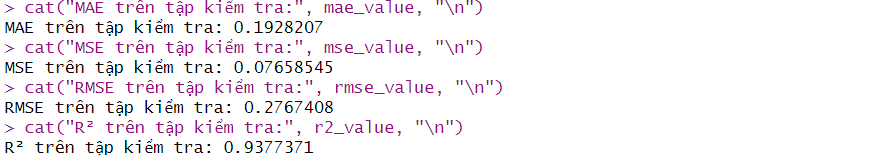
\includegraphics[width=1\linewidth]{images/Screenshot 2025-08-06 013419.png}}
\end{figure}

\textbf{Kết quả các chỉ số đánh giá trên tập kiểm tra thu được như sau:}

\begin{itemize}
    \item \textbf{\textit{Sai số tuyệt đối trung bình MAE}} là 0.1928207, cho thấy độ lệch trung bình giữa giá trị dự đoán và thực tế là khá nhỏ.
    \item \textbf{\textit{Sai số bình phương trung bình MSE}} là 0.07658545, phản ánh mức độ sai lệch tổng thể, với các sai số lớn được phóng đại do tính bình phương.
    \item \textbf{\textit{Căn bậc hai của MSE (RMSE)}} là 0.2767408, cung cấp một thước đo sai số trung bình theo đơn vị của Pixel\_Rate, thể hiện độ chính xác tốt của mô hình.
    \item \textbf{\textit{Hệ số xác định $R^2$}}  là 0.9377371, cho thấy mô hình giải thích được khoảng 93.77\% sự biến thiên của Pixel\_Rate trên tập kiểm tra, chứng tỏ khả năng tổng quát hóa cao.\end{itemize}
    
Nhận xét về kết quả thu được, ta thấy rằng các chỉ số MAE (0.1928207), MSE (0.07658545), và RMSE (0.2767408) đều ở mức thấp, cho thấy mô hình dự đoán chính xác trên tập kiểm tra. RMSE cao hơn một chút so với RMSE từ cross-validation là 0.2767408 so với 0.2678208, nhưng vẫn trong ngưỡng chấp nhận được, phản ánh sự ổn định của mô hình. Giá trị $R^2$ bằng 0.9377371 là rất cao, gần bằng với $R^2$ từ cross-validation là 0.9426636, chứng tỏ mô hình không bị quá khớp (overfitting) và duy trì hiệu suất tốt trên dữ liệu mới.

Sự khác biệt nhỏ giữa các chỉ số trên tập huấn luyện (từ summary(model\_final) và cross-validation) và tập kiểm tra cho thấy mô hình có khả năng tổng quát hóa tốt. Kết quả cho thấy mô hình hồi quy tuyến tính đa biến cho thấy hiệu suất xuất sắc trên tập kiểm tra, xác nhận rằng mô hình có thể được sử dụng đáng tin cậy để dự đoán Pixel\_Rate trên dữ liệu thực tế, với sai số thấp và độ giải thích cao.


\section{Đồ thị Density plot và đồ thị Scatter plot của thực tế so với dự đoán}

Để đánh giá trực quan hiệu suất của mô hình hồi quy tuyến tính đa biến trong việc dự đoán Pixel\_Rate trên tập kiểm tra (test), ta sử dụng density plot và scatter plot so sánh phân bố của giá trị thực tế (Pixel\_Rate) và giá trị dự đoán (predicted\_value). Hai đồ thị này giúp nhận diện sự tương đồng hoặc khác biệt giữa hai phân bố, từ đó đánh giá độ chính xác và xu hướng sai lệch của mô hình.

\subsection{Đồ thị Density plot}

Ta sử dụng mã sau cho đồ thị:

\begin{minted}{r}
# 6.2 Density plot/Scatter plot thực vs dự đoán
# Density plot
test_long <- test %>%
  select(Pixel_Rate, predicted_value) %>%
  rename(Thuc_te = Pixel_Rate, Du_doan = predicted_value) %>%
  pivot_longer(everything(), names_to = "Type", values_to = "Value")

ggplot(test_long, aes(x = Value, fill = Type)) +
  geom_density(alpha = 0.5) +
  scale_fill_manual(values = c("blue", "red")) +
  theme_bw() +
  labs(title = "Thực tế (red) vs Dự đoán (blue) trên tập kiểm tra", x = "Pixel_Rate")
\end{minted}

\begin{figure}[!h]
    \centering
    \fbox{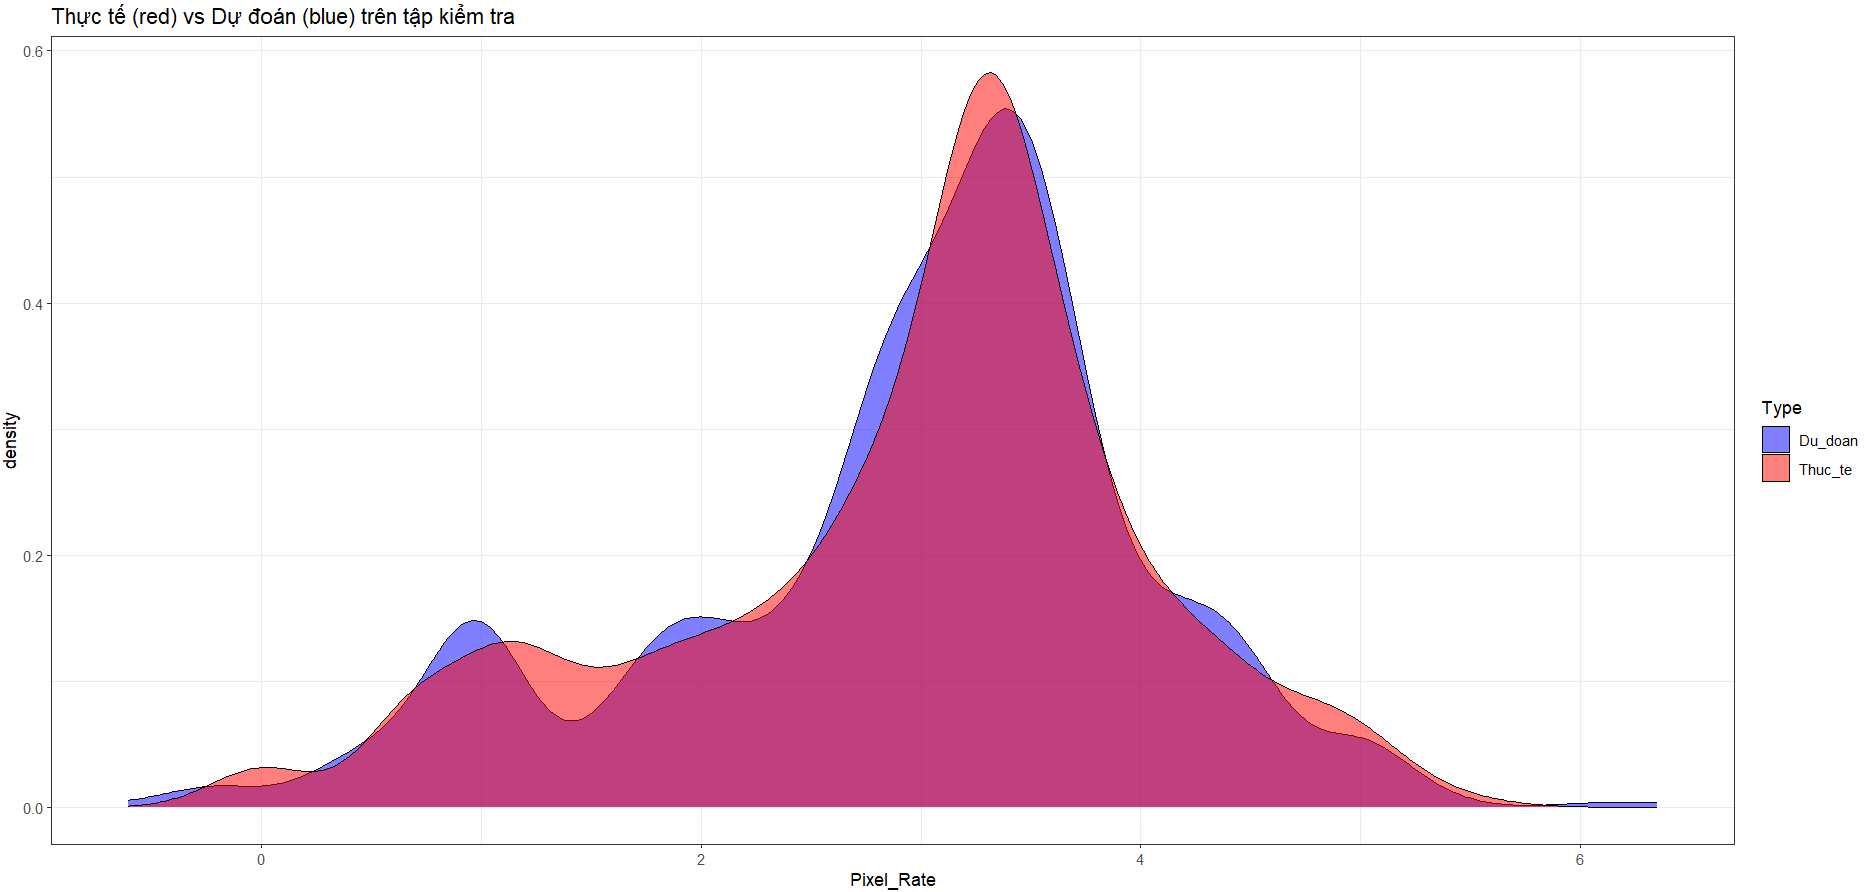
\includegraphics[width=1\linewidth]{images/Screenshot 2025-08-06 013747.png}}
\end{figure}

Trong đó, phần màu đỏ là giá trị thực tế Pixel\_Rate mà ta quan sát được, còn màu xanh chính là giá trị dự đoán được tính toán từ mô hình. Có thể thấy mô hình dự đoán khác tốt với giá trị dự đoán phân bố gần với giá trị thực tế, những phần trùng nhau chiếm diện tích lớn khá lớn và có hình dạng gần tương tự nha, điều này cũng phù hợp với những kết quả thu được trước đó ($R^2$ = 0.9377371, RMSE = 0.2767408). Đường mật độ của giá trị dự đoán có thể hơi mịn hơn do tính chất tổng quát hóa của mô hình, trong khi đường thực tế có thể có các đỉnh hoặc đuôi nhọn hơn do dữ liệu thực tế.

\subsection{Đồ thị Scatter plot}

Ta sử dụng mã sau cho đồ thị:
\begin{minted}{r}
# Scatter plot
ggplot(test, aes(x = Pixel_Rate, y = predicted_value)) +
  geom_point() +
  geom_abline(slope = 1, intercept = 0, col = "red") +
  theme_minimal() +
  labs(title = "Thực tế vs Dự đoán", x = "Thực tế", y = "Dự đoán")
\end{minted}

\begin{figure}[!h]
    \centering
    \fbox{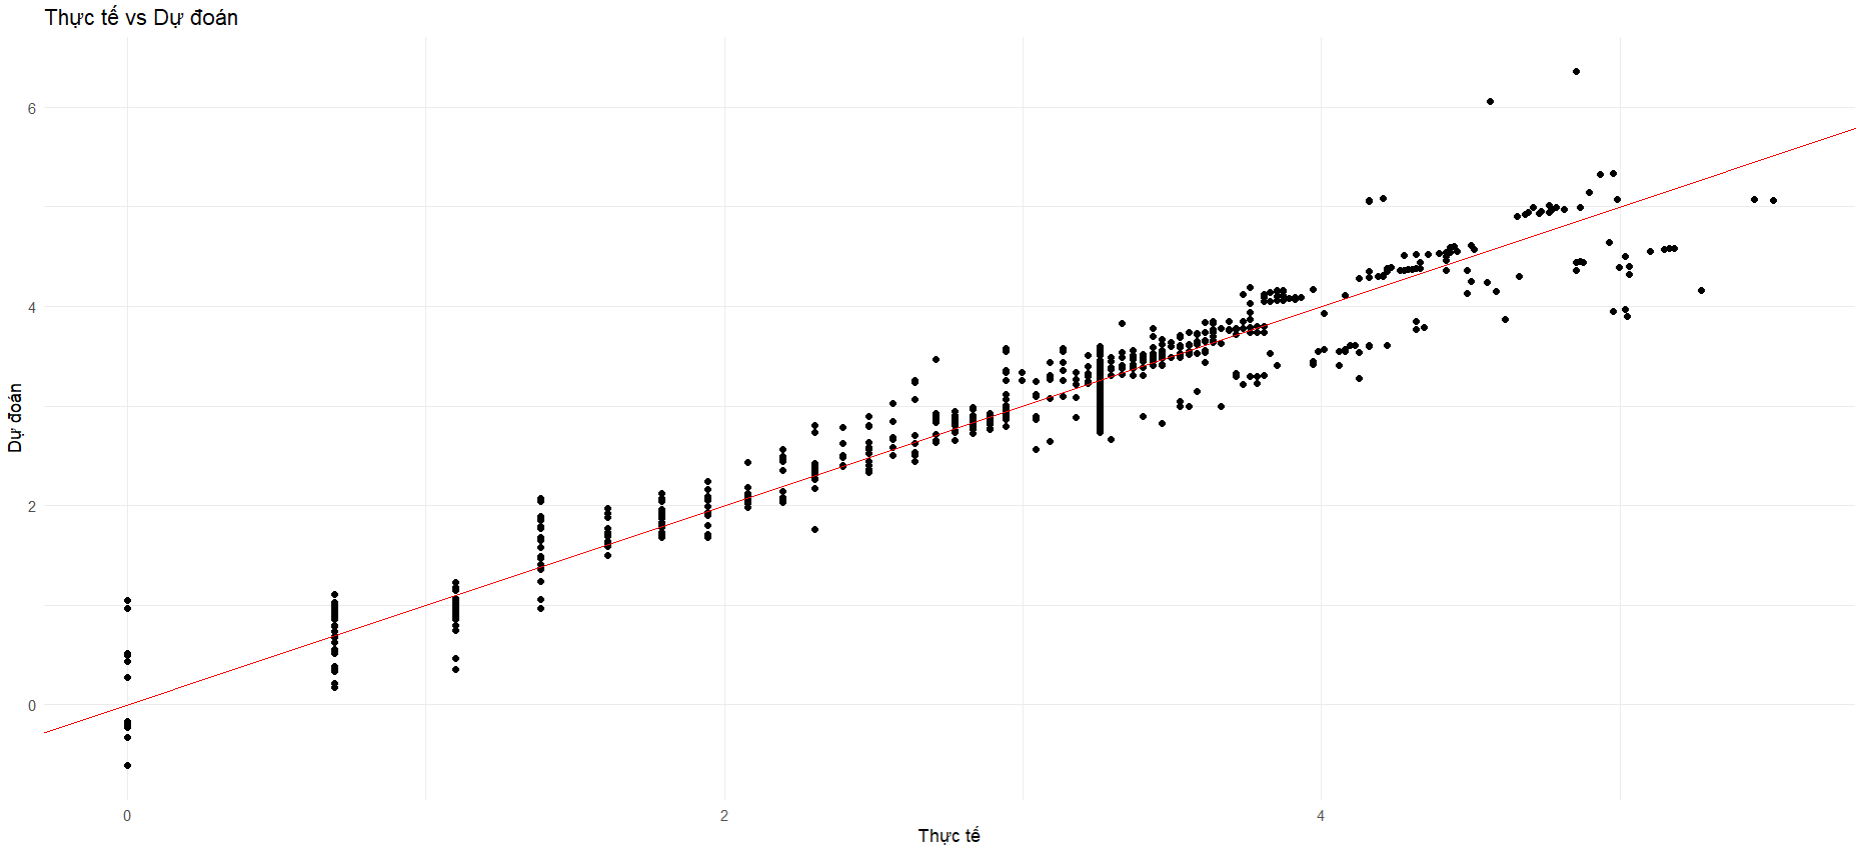
\includegraphics[width=1\linewidth]{images/Screenshot 2025-08-06 013950.png}}
\end{figure}

Với đường chéo màu đỏ thể hiện cho giá trị dự đoán, còn những chấm màu đen chính là giá trị thực tế. Ta dễ dàng thấy được các điểm màu đen tập trung dày đặc gần đường chéo màu đỏ, thể hiện rằng đồ thì có độ chính xác cao, chỉ có một số ít điểm phân tán do sai số.

\section{Prediction intervals cho tương lai}
Từ mô hình hồi quy tuyến tính đa biến mà ta đã xây dựng , ta có thể thực hiện việc dự đoán giá trị của biến Pixel\_Rate thông qua các giá trị của các biến độc lập trong mô hình.

\section{Kịch bản dự báo (giả định khi tăng/giảm biến X)}

Để phân tích tác động của việc thay đổi biến độc lập Core\_Speed đến Pixel\_Rate, ta thực hiện dự báo dựa trên một kịch bản giả định tăng 10\% giá trị Core\_Speed. Quá trình được thực hiện bằng đoạn mã sau:

\begin{minted}{r}
# 6.4 Kịch bản dự báo (giả định tăng/giảm biến X)
scenario_data <- test
scenario_data$Core_Speed <- scenario_data$Core_Speed * 1.1
pred_scenario <- predict(model_final, newdata = scenario_data)
cat("Dự đoán với Core_Speed tăng 10%:\n")
print(summary(pred_scenario))
\end{minted}

\newpage
\begin{figure}[!h]
    \centering
    \fbox{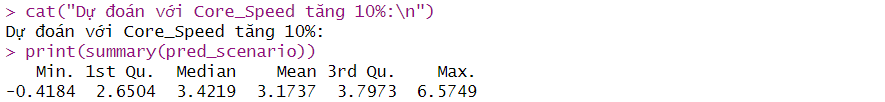
\includegraphics[width=1\linewidth]{images/Screenshot 2025-08-06 014223.png}}
\end{figure}

Giá trị trung bình dự đoán tăng lên 3.1737, so với giá trị trung bình gốc của Pixel\_Rate trên tập test (ước tính khoảng 2.5-2.6 dựa trên dữ liệu trước), cho thấy mức tăng hợp lý. Với hệ số hồi quy Core\_Speed = 0.32165 (từ summary(model\_final)), tăng 10\% Core\_Speed dự kiến làm tăng Pixel\_Rate trung bình khoảng 0.032165 (0.32165 × 0.1), phù hợp với xu hướng quan sát được.